\chapter{Теоретическая часть}
\label{cha:theory}

\section{Определения}

\textbf{Корпус текстов} --- множество подобранных и определённым образом обработанных текстов.

\textbf{Токен} --- элементарная единица разбиения корпуса.

\textbf{Токенизация} --- процесс разбиения корпуса на токены с присвоением им уникальных числовых идентификаторов.

\textbf{Языковая модель} --- распределение $P(w_t | w_1,w_2,w_3,\dots,w_n)$ вероятностей встретить токен $w_t$ в корпусе сразу после $n$ токенов $w_i$, $i\in[1, n]$, идущих подряд, где $w_i \in W \, \forall i$, $W$ --- множество всех токенов корпуса, $n$ --- длина контекста модели.

\textbf{Длина контекста} --- количество $n$ токенов $w_i$, $i\in[0, n]$, предшествующих токену $w_t$, от которых зависит вероятность появления в тексте токена $w_t$.

\textbf{Дообучение} --- процесс обучения уже обученной на некоторых данных модели машинного обучения на новых данных. В случае языковой модели это означает подстройку модели под новое распределение токенов.

\textbf{Перплексия} --- мера схожести двух вероятностных распределений, используемая для оценки качества генерации текста языковой моделью. Перплексия задаётся формулой \ref*{eq:perplexity}.
\begin{equation}
    \label{eq:perplexity}
    \textrm{PP}(W)=\sqrt[n]{\frac{1}{P(w_1,w_2,\dots,w_n)}}
\end{equation}

\section{Постановка задачи}

Дано:
\begin{itemize}
    \item корпус, состоящий из текстов, принадлежащих конкретной предметной области,
    \item предобученная нейросетевая языковая модель, хорошо моделирующая вероятностное распределение слов в естественном языке.
\end{itemize}
Требуется:
\begin{enumerate}
    \item дообучить данную языковую модель на данных из корпуса, получив новую языковую модель, моделирующую распределение вероятностей слов в данном корпусе,
    \item реализовать возможность применения её для генерации новых текстов, принадлежащих предметной области данного корпуса,
    \item создать графический интерфейс для взаимодействия пользователя с моделью,
    \item подготовить получившееся приложение для дистрибуции.
\end{enumerate}

\section{Нейронные сети}

Одной из простейших моделей машинного обучения является однослойный перцептрон. Он позволяет, обучаясь на выборке данных, решать задачу линейной регрессии, то есть, устанавливать зависимость между зависимой переменной $y$ и независимыми переменными $x$ при условии, что между ними существует линейная зависимость, которую можно описать уравнением \ref*{eq:lin_reg}. В нём всегда $x_0\equiv 1$, а $w_0$ называется смещением, так как изменение этой компоненты приводит к увеличению или уменьшению $y$ на постоянное значение.
\begin{equation}
    \label{eq:lin_reg}
    y=\mathbf{w}\cdot\mathbf{x}=w_0x_0+w_1x_1+w_2x_2+\dots+w_nx_n,\quad x_0\equiv 1
\end{equation}

В этом уравнении неизвестными являются компоненты вектора $\mathbf{w}$, найдя которые, можно получить взаимосвязь между $x$ и $y$. Обучающая выборка данных представляет собой матрицу $X$ размера $m \times (n+1)$ наблюдений вектора $\mathbf{x}$ и вектор $\mathbf{y}$ размера $m$, где $y_i=\mathbf{w} \cdot \mathbf{x}_i$, $\mathbf{x}_i$ --- $i$-я строка матрицы $X$, как показано в уравнении \ref*{eq:lin_reg_dataset}.
\begin{equation}
    \label{eq:lin_reg_dataset}
    X\mathbf{w}=
    \left(\begin{matrix}
        x_0^1 & x_1^1 & x_2^1 & x_3^1 & \dots & x_n^1 \\
        x_0^2 & x_1^2 & x_2^2 & x_3^2 & \dots & x_n^2 \\
        x_0^3 & x_1^3 & x_2^3 & x_3^3 & \dots & x_n^3 \\
        x_0^4 & x_1^4 & x_2^4 & x_3^4 & \dots & x_n^4 \\
        \vdots & \vdots & \vdots & \vdots & \ddots & \vdots \\
        x_0^m & x_1^m & x_2^m & x_3^m & \dots & x_n^m
    \end{matrix}\right)
    \left(\begin{matrix}
        w_0 \\
        w_1 \\
        w_2 \\
        \vdots \\
        w_n
    \end{matrix}\right)=
    \left(\begin{matrix}
        y_1 \\
        y_2 \\
        y_3 \\
        y_4 \\
        \vdots \\
        y_m
    \end{matrix}\right)=\mathbf{y}
\end{equation}

Уравнения \ref*{eq:lin_reg_dataset} имеет одно решение относительно $\mathbf{w}$ тогда и только тогда, когда $\rank X = n$. Если $\rank X < n$, уравнение имеет бесконечное число решений, и если $\rank X > n$, уравнение не имеет решений. Но на практике данных обычно больше, чем компонент в векторе $\mathbf{w}$, поэтому используется аппроксимация методом наименьших квадратов, суть которой состоит в том, чтобы путём решения задачи минимизации, показанной в уравнении \ref*{eq:lsm}, найти такую прямую, чтобы функция потерь $L(\mathbf{y},\hat{\mathbf{y}})$ была минимальна.
\begin{equation}
    \label{eq:lsm}
    \begin{cases}
        \mathbf{w} = \arg\min\limits_\mathbf{w} L(\mathbf{y},\hat{\mathbf{y}}), \\
        \hat{\mathbf{y}}=X\mathbf{w}
    \end{cases}
\end{equation}

Из курса математической статистики известно, что лучше всего в данной задаче подходит функция потерь $\MSE$ или средний квадрат ошибки (уравнение \ref*{eq:mse}). При использовании этой функции потерь дисперсия ошибки получается наименьшей.
\begin{equation}
    \label{eq:mse}
    \MSE(\mathbf{y},\hat{\mathbf{y}})=\sum\limits_{i=1}^m(\mathbf{x}_i^T\mathbf{w}-y_i)^2=(X\mathbf{w}-\mathbf{y})^T(X\mathbf{w}-\mathbf{y})
\end{equation}

Минимум функции потерь можно найти градиентными методами, например, методом Adam, так как она дифференцируема, и её производную можно вычислить аналитически (уравнение \ref*{eq:mse_der}). Процесс поиска минимума функции потерь модели называют обучением.
\begin{equation}
    \label{eq:mse_der}
    \frac{\partial\MSE}{\partial \mathbf{w}}(\mathbf{w})=2X^T(X\mathbf{w}-\mathbf{y})
\end{equation}

Если же от модели требуется предсказывать не численные характеристики объектов, а относить их к той или иной группе, то такая задача называется задачей классификации, а модель --- логистической регрессией.

В этом случае требуется не аппроксимировать точки гиперплоскостью, а сделать так, чтобы гиперплоскость отделяла точки одного класса от точек другого. Для этого к выходу линейной регрессии дополнительно применяют функцию с областью значений $[0, 1]$, чтобы выход модели можно было интерпретировать как вероятность принадлежности объекта заданному классу.

\begin{equation}
    \label{eq:sigmoid}
    \sigma(x)=\frac{1}{1+e^{-x}}
\end{equation}

\begin{equation}
    \label{eq:softmax}
    \Softmax(\mathbf{x})=\frac{1}{\sum\limits_{i=1}^n e^{x_i}}
    \left(\begin{matrix}
        e^{x_1} \\
        e^{x_2} \\
        e^{x_3} \\
        \vdots \\
        e^{x_n}
    \end{matrix}\right),\quad \mathbf{x}\in \R^n
\end{equation}

В случае бинарной классификации, то есть, когда класса два, в роли такой функции выступает сигмоида (уравнение \ref*{eq:sigmoid}). Тогда выход модели трактуется как вероятность принадлежности объекта первому классу. Если же классов больше двух, то на выходе модели должен получиться вектор, содержащий столько компонент, сколько в задаче классов, и к нему применяется функция $\Softmax$ (уравнение \ref*{eq:softmax}), выход которой удовлетворяет аксиомам вероятности \ref*{eq:prob_axioms}.
\begin{equation}
    \label{eq:prob_axioms}
    \begin{cases}
        \mathbf{y}=\left(\begin{matrix}
            y_1 & y_2 & y_3 & \dots & y_n
        \end{matrix}\right)^T \\
        y_i \in [0, 1]\,\forall i\in[1, n], \\
        \sum\limits_{i=1}^n y_i = 1
    \end{cases}
\end{equation}

В задаче классификации используется функция потерь, называемая перекрёстной энтропией (уравнение \ref*{eq:ce_loss}). В случае бинарной классификации она представляется в виде \ref*{eq:bce_loss}.
\begin{equation}
    \label{eq:ce_loss}
    \CE(\mathbf{y},\hat{\mathbf{y}})=-\sum\limits_{i=1}^n y_i \ln \hat{y}_i
\end{equation}
\begin{equation}
    \label{eq:bce_loss}
    \BCE(y,\hat{y})=-y \ln \hat{y} - (1-y)\ln (1-\hat{y})
\end{equation}

Модели линейной и логистической регрессии позволяют строить аппроксимации только гиперплоскостями. Чтобы иметь возможность аппроксимировать нелинейные зависимости в данных, их применяют последовательно, перемежая нелинейными функциями, например, как в уравнении \ref*{eq:nn_sample}. Тогда функция $f(x)$ называется нейронной сетью, а линейные модели, из которых она состоит --- её слоями. Параметры, или веса, нейронной сети, состоят из параметров всех её слоёв, а оптимизируются они так же, градиентными методами.
\begin{equation}
    \label{eq:nn_sample}
    f(x)=\sigma(\dots \sigma(\sigma(xw_1)w_2)w_3 \dots)
\end{equation}

Функции, перемежающие применения линейных слоёв, могут быть любыми кусочно-гладкими нелинейными функциями, а на то, какие операции производятся над слоями внутри нейронной сети, накладывается только одно ограничение: функция $f(x)$ должна оставаться кусочно-гладкой, чтобы можно было искать минимум функции потерь градиентными методами.

\section{Градиентные методы оптимизации}

Минимум функции потерь при обучении нейронных сетей обычно ищется градиентными методами, которые хорошо себя зарекомендовали в решении задач на оптимизацию дифференцируемых функций.

Суть этой группы методов хорошо иллюстрировать на примере простейшего из них --- градиентного спуска.

Пусть имеется задача, представленная в уравнении \ref*{eq:grad_desc_problem}.
\begin{equation}
    \label{eq:grad_desc_problem}
    \begin{cases}
        L(\mathbf{w}): \R^n \rightarrow \R, \\
        \nabla L(\mathbf{w}) = \left(\begin{matrix}
            \frac{\partial L}{\partial w_1}(w_1) \\
            \frac{\partial L}{\partial w_2}(w_2) \\
            \frac{\partial L}{\partial w_3}(w_3) \\
            \vdots \\
            \frac{\partial L}{\partial w_n}(w_n)
        \end{matrix}\right), \\
        L(\mathbf{w}) \rightarrow \min\limits_\mathbf{w}
    \end{cases}
\end{equation}

Требуется найти минимум дифференцируемой функции $n$ переменных. Как известно из курса математического анализа, градиент функции нескольких переменных, вычисленный в конкретной точке --- это вектор, указывающий направление наискорейшего возрастания функции в этой точке. Значит, чтобы найти минимум, двигаясь из какой-либо начальной точки, нужно перемещаться в направлении, противоположном градиенту. Эту идею реализует градиентный спуск (уравнение \ref*{eq:grad_desc_algo}).
\begin{equation}
    \label{eq:grad_desc_algo}
    \mathbf{w}^{t+1}=\mathbf{w}^t-\alpha\nabla L(\mathbf{w})
\end{equation}

Делая шаги длины $\alpha$ в направлении антиградиента функции, с увеличением $t$ алгоритм приближается к минимуму.

Но у этого алгоритма есть ряд проблем, связанных со скроростью сходимости. Наглядный пример приведён на рисунке \ref*{fig:grad_desc_problem}. В нём целевая функция представляет собой вытянутый параболоид, и градиентный спуск в этом случае делает шаги неоптимальным образом, двигаясь к точке минимума очень медленно.

\begin{figure}
    \centering
    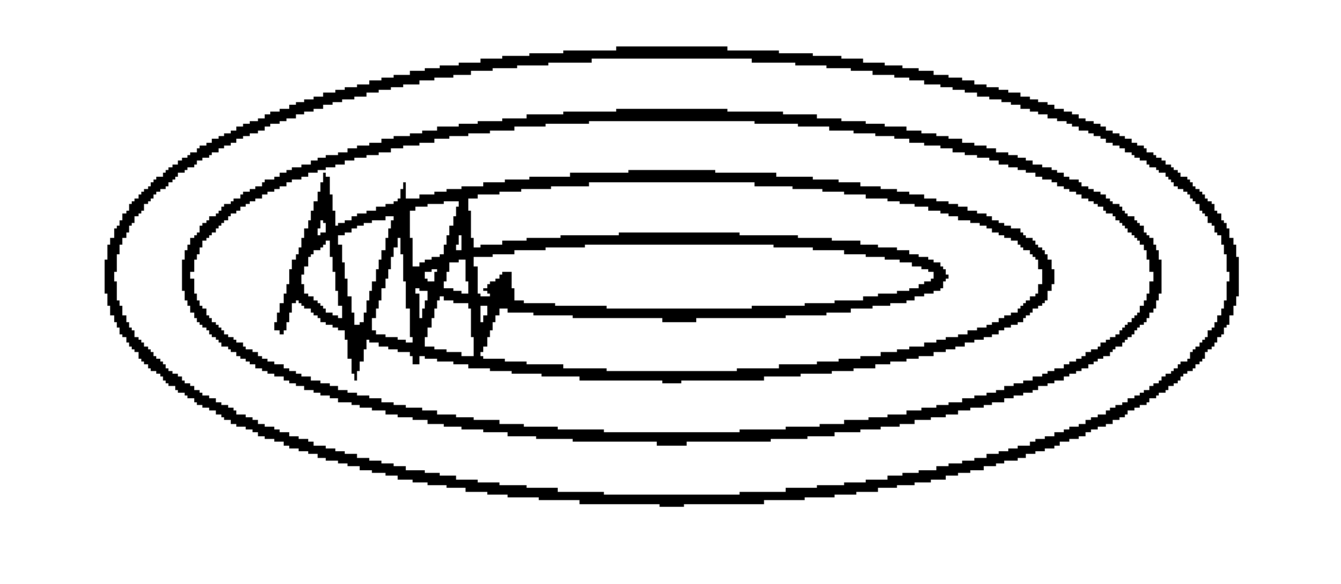
\includegraphics[width=0.5\textwidth]{../inc/images/gradient_descend_problem.png}
    \caption{Проблема долгой сходимости простого градиентного спуска}
    \label{fig:grad_desc_problem}
\end{figure}

Одним из решений этой проблемы является введение физических характеристик для точки, двигающейся по поверхности целевой функции. Например, в методе Adam (англ. --- Adaptive Moment Estimation) вводятся масса и скорость, моделируя движение шарика вниз по неровной поверхности.

Другая проблема состоит в том, что фиксированный шаг градиентного спуска может мешать оптимизации функции по некоторым координатам. В методе Adam это решается путём введения специальных весов, уменьшающих шаг по координатам, которые часто изменяются. Метод Adam описывается уравнениями \ref*{eq:adam}.
\begin{equation}
    \label{eq:adam}
    \begin{cases}
        \mathbf{m}^t=\beta_1\mathbf{m}^{t-1}+(1-\beta_1)\nabla L(\mathbf{w}) \\
        \mathbf{v}^t=\beta_2\mathbf{v}^{t-1}+(1-\beta_2)(\nabla L(\mathbf{w}))^2 \\
        \hat{\mathbf{m}}^t=\frac{\mathbf{m}^t}{1-\beta_1^t} \\
        \hat{\mathbf{v}}^t=\frac{\mathbf{v}^t}{1-\beta_2^t} \\
        \mathbf{w}^{t+1}=\mathbf{t}-\frac{\alpha}{\sqrt{\hat{\mathbf{v}}^t}+\varepsilon}\hat{\mathbf{m}}^t \\
        \mathbf{m}^0=\mathbf{0},\quad\mathbf{v}^0=\mathbf{0}
    \end{cases}
\end{equation}

Параметры $\beta_1$, $\beta_2$, $\varepsilon$ и $\alpha$ задаются по усмотрению пользователя в зависимости от решаемой задачи.

На сегодняшний день Adam является одним из лучших алгоритмов оптимизации, показывающих наименьшее время сходимости при обучении нейронных сетей на разнообразных данных \cite{art:optimizers}.
